\documentclass[a4paper,10pt]{article}

\usepackage[activeacute]{babel}
\usepackage[utf8]{inputenc}
\usepackage{bookman}
\usepackage{color}
\usepackage{graphicx}
\usepackage{anysize}
\usepackage{multicol}
\usepackage[pdftex=true,colorlinks=true,linkcolor=black,urlcolor=blue]{hyperref}

\marginsize{1.5cm}{1.5cm}{1.5cm}{1.5cm}
\newcommand{\HRule}{\rule{\linewidth}{0.5mm}}
\newcommand{\tab}{\hspace*{0.5cm}}

\date{}

\pagenumbering{arabic}
\setcounter{page}{1}

\begin{document}

% ===================================== MEMBRETE ===================================== %
\begin{center}
  \textsc {
    Universidad Simón Bolívar \\[0cm]
    Departamento de Computaci\'on y Tecnolog\'ia de la Informaci\'on \\[0cm]
    CI5438 - Inteligencia Artificial I \\[0cm]
    Trimestre Abril - Julio 2021 \\[0cm]
    Prof. Carlos Infante \\[0cm]
    Amin Arriaga 16-10072, David Segura 13-11341, Wilfredo Graterol 15-10639
  }
  \HRule \\[0.4cm]
  {\Large \textbf{Scheduling Problem as CNF}} \\[0.4cm]
  \textsc{
    \today
  }
  \HRule
\end{center}

\section{Formulaci\'on}
  Sea $\mathcal{E}$ el conjunto de equipos, $\mathcal{F}$ el conjunto de fechas 
  disponibles y $\mathcal{H}$ el conjunto de horarios disponibles tal que 
  $E = |\mathcal{E}|$, $F = |\mathcal{F}|$ y $H = |\mathcal{H}|$. Entonces, las 
  variables de nuestro CNF se identifican de la forma $(e_i,e_j,h,f)$ donde 
  $e_i,e_j \in \mathcal{E}$ con $e_i \neq e_j$, $h \in \mathcal{H}$ y 
  $f \in \mathcal{F}$ e indican que el equipo $e_i$ juega como local en contra 
  del equipo $e_j$ como visitante en la fecha $f$ y hora $h$. Por lo tanto, 
  nuestro CNF tiene $E(E-1)FH$ variables, y las enumeramos como\footnote{Los
  booleanos son tratados como 1 para \textit{True} y 0 para \textit{False}}: \\

  \noindent
  $ENUM(e_i, e_j, h_k, f_l) = i - (i > j)*j - (j > i)(j - 1) + E*j + $
  $E(E - 1)*k + E(E - 1)H*l$  \\ 

  \noindent
  donde \\

  \noindent
  $0 \leq i, j < E$, $0 \leq l < H$ y $0 \leq k < F$
  
  \subsection{Restricciones y Clausuras}
    \begin{itemize}
      \item Todos los participantes deben jugar dos veces con cada uno de los 
      otros participantes, una como "visitantes" y la otra como "locales". \\

      $(\forall e_i, e_j \in \mathcal{E} \: | \: e_i \neq e_j : (\exists f \in $
      $\mathcal{F}, h \in \mathcal{H} \: | \: : (e_i, e_j, f, h)) \: )$ \\

      Con un total de $E(E-1)$ clausuras tal que cada una esta conformada 
      por $FH$ \'atomos.\\

      \item Dos juegos no pueden ocurrir al mismo tiempo.\\
      
      $(\forall f \in \mathcal{F}, h \in \mathcal{H}, e_i, e_j \in \mathcal{E} $
      $\: | \: e_i \neq e_j :$\\
      \tab $(\forall e_m', e_n' \in \mathcal{E} \: | \: e_m' \neq e_n' \wedge $
      $(m > i \vee (m = i \wedge n > j) : $\\
      \tab \tab $\neg (e_i, e_j, h, f) \vee \neg (e_m', e_n', h, f)$ \\
      \tab $)$\\
      $)$ \\

      Con un total de $\frac{1}{2}E(E-1)(E(E-1)-1)FH$ clausuras con 2 
      \'atomos cada una.\\


      \item Un participante puede jugar a lo sumo una vez por día. \\
      
      $(\forall e, e_i', e_j' \in \mathcal{E}, f \in \mathcal{F}, h, h' \in \mathcal{H}$
      $ \: | \: e \neq e_i' \wedge e \neq e_j' \wedge i < j \wedge h \neq h' : $\\
      \tab $(\neg (e, e_i', f, h) \vee \neg (e, e_j', f, h')) \: \wedge \: $
      $(\neg (e_i', e, f, h) \vee \neg (e_j', e, f, h'))$\\
      $) \: \wedge $\\
      $(\forall e, e_i', e_j' \in \mathcal{E}, f \in \mathcal{F}, h, h' \in \mathcal{H}$
      $ \: | \: e \neq e_i' \wedge e \neq e_j' \wedge e_i' \neq e_j' \wedge h \neq h' : $\\
      \tab $\neg (e, e_i', f, h) \vee \neg (e_j', e, f, h')$\\
      $) \: \wedge $\\
      $(\forall e_i, e_j \in \mathcal{E}, f \in \mathcal{F}, h_m, h_n \in $
      $\mathcal{H} \: | \: i < j \wedge m < n : $\\
      \tab $(\neg (e_i, e_j, h_m, f) \vee \neg (e_i, e_j, h_n, f)) \: \wedge $
      $\: (\neg (e_j, e_i, h_m, f) \vee \neg (e_j, e_i, h_n, f)) \: \wedge \: $\\
      \tab $(\neg (e_i, e_j, h_m, f) \vee \neg (e_j, e_i, h_n, f)) \: \wedge $
      $\: (\neg (e_j, e_i, h_m, f) \vee \neg (e_i, e_j, h_n, f))$\\
      $)$\\

      Con un total de $E(E-1)(E-2)FH(H-1) \: + \: E(E-1)(E-2)FH(H-1) \:$
      $ + \: E(E-1)FH(H-1)$ 
      clausuras con 2 \'atomos cada una.


      \item Un participante no puede jugar de \textit{visitante} en dos días 
      consecutivos, ni de \textit{local} dos días seguidos.\\

      $(\forall e, e_i', e_j' \in \mathcal{E}, f_k, f_{k+1} \in \mathcal{F}, h, h'$
      $ \in \mathcal{H} \: | \: e \neq e_i' \wedge e \neq e_j' \wedge e_i' \neq e_j':$\\
      \tab $(\neg (e, e_i', h, f_k) \vee \neg (e, e_j', h', f_{k+1})) \: \wedge \: $
      $(\neg (e_i', e, h, f_k) \vee \neg (e_j', e, h', f_{k+1}))$\\
      $)$\\

      Con un total de $2E(E-1)(E-2)(F-1)H^2$ de clausuras con 2 \'atomos cada una.\\


      \item Todos los juegos deben empezar en horas "en punto" (por ejemplo, 
      las 13:00:00 es una hora válida pero las 13:30:00 no). Esta restricci'on
      no forma parte de las condiciones para las clausuras.

      \item Todos los juegos deben ocurrir entre una fecha inicial y una fecha final 
      especificadas. Pueden ocurrir juegos en dichas fechas. Esta restricci'on
      no forma parte de las condiciones para las clausuras.

      \item Todos los juegos deben ocurrir entre un rango de horas especificado, el 
      cuál será fijo para todos los días del torneo. Esta restricci'on no forma 
      parte de las condiciones para las clausuras.

      \item A efectos prácticos, todos los juegos tienen una duración de dos horas.
      Esta restricci'on no forma parte de las condiciones para las clausuras.\\
      
      Estas \'ultima 4 condiciones definen los valores de $\mathcal{F}$ y 
      $\mathcal{H}$. Usando la restricci\'on de las fechas, identificamos las 
      fechas en orden cronol\'ogico en el rango $[0,F)$ siendo $F$ tambi\'en el 
      n\'umero de d\'ias entre las fechas inicial y final. An\'alogamente, usando 
      las restricciones relacionadas con las horas, podemos calcular cuantos 
      partidos se pueden realizar al d\'ia y en que horarios espec\'ificos, luego 
      podemos identificar cada bloque del horario en orden cronol\'ogico en el 
      rango $[0, H)$, donde $H$ tambi\'en es el n\'umero de partidos que se pueden 
      realizar al d\'ia.
    \end{itemize}

    En total se tienen $O(E^3FH(E + H))$ clausuras, por lo tanto, el factor principal
    en la complejidad del problema es precisamente el n\'umero de equipos, seguido 
    por el n\'umero de horas por d\'ia.

\section{Formulaci\'on V2}  
  Sea $\mathcal{E}$ el conjunto de equipos, $\mathcal{F}$ el conjunto de fechas 
  disponibles y $\mathcal{H}$ el conjunto de horarios disponibles tal que 
  $E = |\mathcal{E}|$, $F = |\mathcal{F}|$ y $H = |\mathcal{H}|$. Entonces, 
  definimos dos tipos de variables: 

  \subsection{Variables de tipo 1}
    Las variables de tipo 1 se definen como $(e_i,e_j,h,f)$ donde 
    $e_i,e_j \in \mathcal{E}$ con $e_i \neq e_j$, $h \in \mathcal{H}$ y 
    $f \in \mathcal{F}$ e indican que el equipo $e_i$ juega como local en contra 
    del equipo $e_j$ como visitante en la fecha $f$ y hora $h$. Por lo tanto, 
    hay $E(E-1)FH$ variables de tipo 1, y las enumeramos como\footnote{Los 
    booleanos son tratados como 1 para \textit{True} y 0 para \textit{False}} \\

    \noindent
    $ENUM_1(e_i, e_j, h_k, f_l) = i - (i > j)*j - (j > i)(j - 1) + E*j + $
    $E(E - 1)*k + E(E - 1)H*l$  \\ 

    \noindent
    donde \\

    \noindent
    $0 \leq i, j < E$, $0 \leq k < F$ y $0 \leq l < H$\\
  
  \subsection{Variables de tipo 2}
    Las variables de tipo 2 son de la forma $(e,t,h,f)$ donde $e_ \in \mathcal{E}$, 
    $f \in \mathcal{F}$, $t \in \{v, l\}$ y $h \in \mathcal{H}$ e indican que el 
    equipo $e$ juega como $t$ (local o visitante) en la fecha $f$ y hora $h$. Por 
    lo tanto, hay $2E F H$ variables de tipo 2, y las enumeramos 
    como: \\

    \noindent
    $ENUM_2(e_i, t, h_j, f_k) = E (E-1) F H + 1 + i + E * (t == v) + 2 E*j$
    $ + 2 E H*k$  \\ 

    \noindent
    donde \\

    \noindent
    $0 \leq i < E$, $0 \leq k < F$ y $0 \leq l < H$\\

    \noindent
    as\'i, nuestro CNF tiene un total de $E(E+1)FH$ variables.

  \subsection{Restricciones y Clausuras}
    \begin{itemize}
      \item Todos los participantes deben jugar dos veces con cada uno de los 
      otros participantes, una como "visitantes" y la otra como "locales". \\

      $(\forall e_i, e_j \in \mathcal{E} \: | \: e_i \neq e_j : (\exists f \in$
      $ \mathcal{F}, h \in \mathcal{H} \: | \: : (e_i, e_j, f, h)) \: )$ \\

      Con un total de $E(E-1)$ clausuras tal que cada una est\'a conformada 
      por $FH$ \'atomos. Esta restricci\'on fue la causante de tener que usar
      dos tipos de variables, pues si s\'olo tuvi\'eramos las de tipo 2, entonces 
      la restricci\'on quedar\'ia de la forma:\\ 

      $(\forall e_i, e_j \in \mathcal{E} \: | \: e_i \neq e_j : $\\
      \tab $(\exists f \in \mathcal{F}, h \in \mathcal{H} \: | \: : $\\
      \tab \tab $ (e_i, l, f, h) \wedge (e_j, v, f, h) $ \\
      \tab $)$ \\
      $)$ \\

      Notemos que hay conjunciones dentro de las cl\'ausuras, lo cual hace que 
      ya no sea CNF, por lo tanto, usando la propiedad distirbutiva entre 
      conjunciones y disyunciones, reescribimos la restricci\'on anterior como\\

      $(\forall e_i, e_j \in \mathcal{E} \: | \: e_i \neq e_j : $\\
      \tab $(\forall A \in \mathcal{P}(\mathcal{F} \times \mathcal{H}) \: | \: A $
      $\neq \emptyset \wedge A \neq \mathcal{F} \times \mathcal{H}: $\\
      \tab \tab $(\exists (f, h) \in A \: | \: : (e_i, l, f, h)) \: \vee$ \\ 
      \tab \tab $(\exists (f', h') \in (\mathcal{F} \times \mathcal{H} - A) \: $
      $| \: : (e_j, v, f', h'))$\\
      \tab $)$\\
      $)$\\

      D\'andonos un total de $E(E-1)(2^{FH} - 2)$ clausuras con $FH$ 
      \'atomos cada una. Tener un n\'umero exponencial de clausuras hace que resolver 
      el problema se vuelva inviable. Usando solo 8 d\'ias con 3 partidos diarios
      y 4 equipos nos dar\'ia un total de 201,326,568 clausuras solo para esta 
      restricci\'on.\\
      
      \item Equivalencia entre las variables de tipo 1 y de tipo 2. La variable 
      $(e_i, e_j, h, f)$ es \verb|True| si y solo si $(e_i, l, h, f) \: \wedge $
      $(e_j, v, h, f)$ es \verb|True|. \\

      $(\forall e_i, e_j \in \mathcal{E}, h \in \mathcal{H}, f \in \mathcal{F} \: |$
      $ \: e_i \neq e_j :$\\
      \tab $(\neg (e_i, e_j, h, f) \vee (e_i, l, h, f)) \: \wedge$\\
      \tab $(\neg (e_i, e_j, h, f) \vee (e_j, v, h, f)) \: \wedge$\\
      \tab $(\neg (e_i, l, h, f) \vee \neg (e_j, v, h, f) \vee (e_i, e_j, h, f))$\\
      $)$\\

      D\'andonos un total de $2E(E-1)HF$ clausuras de 2 \'atomos cada una 
      m\'as $E(E-1)HF$ clausuras de 3 \'atomos cada una.
      


      \item Dos juegos no pueden ocurrir al mismo tiempo.\\
      
      $(\forall e_i, e_j \in \mathcal{E}, f \in \mathcal{F}, h \in \mathcal{H} \: $
      $| \: i < j: $\\
      \tab $(\neg (e_i, l, f, h) \vee \neg (e_j, l ,f, h)) \: \wedge \: $
      $(\neg (e_i, v, f, h) \vee \neg (e_j, v ,f, h)))$\\
      $)$\\

      D\'andonos un total de $E(E-1)FH$ clausuras de 2 \'atomos cada una.\\ 

      \item Un participante puede jugar a lo sumo una vez por día.\\
      
      $(\forall e \in \mathcal{E}, f \in \mathcal{F}, h_i, h_j \in \mathcal{H} $
      $\: | \: i < j : $\\
      \tab $(\neg (e, l, f, h_i) \vee \neg (e, l, f, h_j)) \: \wedge \: $
      $(\neg (e, l, f, h_i) \vee \neg (e, v, f, h_j)) \: \wedge \: $ \\
      \tab $(\neg (e, v, f, h_i) \vee \neg (e, l, f, h_j)) \: \wedge \: $
      $(\neg (e, v, f, h_i) \vee \neg (e, v, f, h_j))$ \\
      $)$\\

      D\'andonos un total de $2EFH(H-1)$ clausuras de 2 \'atomos cada una.\\

      \item Un participante no puede jugar de \textit{visitante} en dos días 
      consecutivos, ni de \textit{local} dos días seguidos.\\

      $(\forall e \in \mathcal{E}, f_i \in \mathcal{F}, h, h' \in \mathcal{H} \: $
      $| \: i < F-1 : $ \\
      \tab $(\neg (e, l, f_i, h) \vee \neg (e, l, f_{i+1}, h')) \: $
      $\wedge \: (\neg (e, v, f_i, h) \vee \neg (e, v, f_{i+1}, h'))$\\
      $)$\\

      D\'andonos un total de $2E(F-1)H^2$ clausuras de 2 \'atomos cada una.

      \item Todos los juegos deben empezar en horas "en punto" (por ejemplo, 
      las 13:00:00 es una hora válida pero las 13:30:00 no). Esta restricci'on
      no forma parte de las condiciones para las clausuras.

      \item Todos los juegos deben ocurrir entre una fecha inicial y una fecha final 
      especificadas. Pueden ocurrir juegos en dichas fechas. Esta restricci'on
      no forma parte de las condiciones para las clausuras.

      \item Todos los juegos deben ocurrir entre un rango de horas especificado, el 
      cuál será fijo para todos los días del torneo. Esta restricci'on no forma 
      parte de las condiciones para las clausuras.

      \item A efectos prácticos, todos los juegos tienen una duración de dos horas.
      Esta restricci'on no forma parte de las condiciones para las clausuras.\\
      
      Estas \'ultima 4 condiciones definen los valores de $\mathcal{F}$ y 
      $\mathcal{H}$. Usando la restricci\'on de las fechas, identificamos las 
      fechas en orden cronol\'ogico en el rango $[0,F)$ siendo $F$ tambi\'en el 
      n\'umero de d\'ias entre las fechas inicial y final. An\'alogamente, usando 
      las restricciones relacionadas con las horas, podemos calcular cuantos 
      partidos se pueden realizar al d\'ia y en que horarios espec\'ificos, luego 
      podemos identificar cada bloque del horario en orden cronol\'ogico en el 
      rango $[0, H)$, donde $H$ tambi\'en es el n\'umero de partidos que se pueden 
      realizar al d\'ia.
    \end{itemize}

    En total se tienen $O(E * F * H * (E + H))$ clausuras, por lo tanto, los factores
    principales que determinan la complejidad del problema es el n\'umero de equipos 
    y partidos diarios.

  
\section{Estructura del repositorio}
  El repositorio del proyecto tiene la siguiente estructura de arbol:

  \begin{verbatim}
    proyecto-3-ci5437/
    |--- benchmarks/...
    |--- bin/...
    |--- Makefile
    |--- README.md
    +--- src/
        |--- benchmarksGen.py
        |--- closuresGen.cpp
        |--- closuresGenV2.cpp
        |--- glucose/...
        |--- L_informe/...
        |--- main.py
        |--- verifyClosures.py
        +--- verifyClosuresV2.py
  \end{verbatim}

  \noindent
  donde 

  \begin{itemize}
    \item \verb|benchmarks/| contiene los casos de prueba en formato JSON junto
    a sus soluciones (en caso de haberla) en archivos \verb|.ics|.

    \item \verb|bin/| contiene los archivos binarios.
    
    \item \verb|glucose/| contiene toda la implementaci\'on del SAT Solver 
    \href{https://www.labri.fr/perso/lsimon/glucose/}{Glucose}.

    \item \verb|L_informe/| contiene los archivos de \LaTeX \hspace{0.075cm} 
    necesarios para generar este informe.

    \item \verb|benchmarksGen.py| es el generador de casos de prueba.

    \item \verb|closuresGen.cpp| y \verb|closuresGenV2.cpp| son el c\'odigo 
    fuente para el generador de archivos \verb|.cnf| usando la formulaci\'on 
    original y V2 respectivamente.

    \item \verb|verifyClosures.cpp| y \verb|verifyClosuresV2.cpp| son el c\'odigo 
    fuente para verificar que las clausuras codificadas no se repiten y su n\'umero 
    coincide con el calculado te\'oricamente usando la formulaci\'on original 
    y V2 respectivamente.

    \item \verb|main.py| se encarga de leer el archivo JSON, generar su correspondiente
    archivo \verb|.cnf|, ejecutar el SAT Solver y traducir la soluci\'on en un 
    archivo \verb|.ics|.
  \end{itemize}


\section{Compilaci\'on y ejecuci\'on}
  Los archivos que necesitan ser compilados son el generador de CNF y Glucose. Para 
  el primero, debemos ejecutar lo siguiente mientras nos encontramos en el directorio 
  raiz del repositorio:

  \begin{center}
    \verb@make closuresGen  @ \'o \verb@  make closuresGenV2@
  \end{center}

  \noindent
  Esto nos crear\'a el archivo binario para la generaci\'on de CNF dentro del directorio 
  \verb|bin/|. Mientras que para Glucose mantenemos el archivo binario almacenado en 
  \verb|bin/| ya que la implementaci\'on del SAT Solver no ser\'a modificada por nosotros,
  as\'i que no es necesario compilarlo en cada ocasi\'on. Luego, para la ejecuci\'on de 
  \verb|main.py| se debe seguir la siguiente sintaxis:

  \begin{center}
    \verb|python main.py  JSON  CLOSURES_GEN  SAT_SOLVER  OUTPUT_ICS|
  \end{center}

  \noindent
  donde 

  \begin{itemize}
    \item \verb|JSON| es el archivo que contiene el problema.
    \item \verb|CLOSURES_GEN| es el binario generador de CNF.
    \item \verb|SAT_SOLVER| es el binario para resolver el CNF. 
    \item \verb|OUTPUT_ICS| es el archivo \verb|ics| donde se almacenar\'a la soluci\'on.
  \end{itemize}

  \noindent
  Por ejemplo si nos encontramos en el directorio raiz del repositorio, una posible ejecuci\'on 
  puede ser 

  \begin{verbatim}
    python src/main.py benchmarks/benchmark_e=4.json \
      bin/closuresGenV2.out \
      bin/glucose \  
      benchmarks/benchmark_e=4.ics
  \end{verbatim}

  \subsection{Generador de Casos de Prueba}
    Para generar casos de prueba de forma autom\'atica puede ejecutar el script 
    \verb|benchmarksGen.py| siguiendo la sintaxis:

    \begin{center}
      \verb|python benchmarksGen.py TEAMS DAYS DAILY_MATCHES|
    \end{center}

    Esto crear\'a un archivo JSON siguiendo la sintaxis de los torneos dado en el 
    README tal que el nombre del torneo es \textit{POMAC}, la fecha de inicio es 
    \textit{1999-11-28}, la fecha final es igual a la inicial mas \verb|DAYS| d\'ias,
    la hora inicial es a las \textit{00:00:00}, la hora final es igual a la inciial 
    m\'as 2 veces \verb|DAILY_MATCHES| horas y los equipos ser\'an desde \textit{T0}
    hasta \textit{TN} donde \textit{N} es igual a \verb|TEAMS|. El nombre del archivo 
    ser\'a \verb|benchmark_E<TEAMS>H<DAILY_MATCHES>F<DAYS>.json|. Por ejemplo si se 
    ejecuta:

    \begin{center}
      \verb|python benchmarksGen.py 15 55 7|
    \end{center}

    Se obtendr\'a el archivo \verb|benchmark_E15H7F55.json|


\section{Resultados y Conlusiones}
  Los casos de prueba se definen por el n\'umero de equipos que participar\'an, 
  el n\'umero de d\'ias que durar\'a el torneo y el n\'umero m\'aximo de partidos
  diarios. Decidimos probar tanto la formulaci\'on V1 como V2 y comparar sus 
  desempe\~nos. En caso de que alguno de estos dos no haya terminado un caso de 
  prueba, se coloca una nota explicando la raz\'on por la que se cancel\'o su 
  ejecuci\'on. En la \textit{Figura 1} se encuentra el resumen de ejecuci\'on de 
  cada caso de prueba.\\ 

  No se podr\'ia decir a partir de los casos de pruebas cual versi\'on de la 
  formulaci\'on es mejor, ya que no hay una que tenga un mejor rendimiento de 
  forma constante. Sin embargo, se puede notar que si la holgura (diferencia entre 
  el n\'umero de d\'ias por el n\'umero de enfrentamientos diarios menos el n\'umero 
  de partidos necesarios, es decir, $E * (E-1)$) es muy ajustada, V1 tiende a tener 
  un mejor rendimiento, mientras que al aumentar la holgura, V2 mejora 
  considerablemente, llegando a tardar pocos segundos para casos de prueba grande.
  Tambi\'en podemos notar que a partir de cierto tama\~no en los casos de prueba,
  V1 se vuelve inviable debido al uso de memoria. Esto se debe a la cantidad de 
  casos de prueba que genera. Por ejemplo, para $(19, 90, 9)$, V1 genera alrededor
  de 23 millones de clausuras, mientras que V2 s\'olo genera 565 mil. Suponiendo que 
  cada clausura ocupe 64 bytes (por poner un n\'umero), entonces las 23M de 
  clausuras ocupar\'ian m\'as de 1GB de memoria. Para el caso $(20, 110, 10)$ ni
  siquiera vale la pena hacer el c\'alculo. Sin embargo, V2 puede llegar a ser muy ineficiente cuando la holgura es muy 
  ajustada, como se nota en los casos de prueba donde no termina. \\

  Se puede concluir que si el caso de prueba es lo suficientemente peque\~no
  (menos de 19 equipos) y la holgura es poca, entonces se debe usar V1, en caso 
  contrario V2. \\


\begin{figure*}[t!]
  \centering
  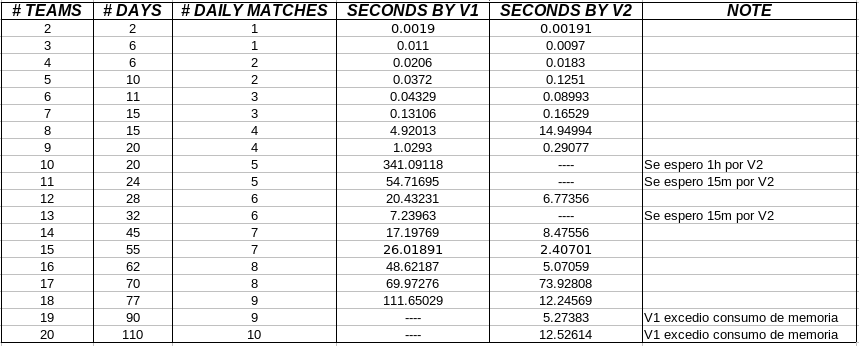
\includegraphics[scale=2.5]{resultados.png}\\
  \small{\textit{Figura 1. Resultados de los casos de prueba aplicados a ambas 
  versiones de la Formulaci\'on.}}\\
\end{figure*}



\end{document}